\documentclass[tikz,border=12pt]{standalone}
\usepackage[T1]{fontenc}
\usepackage{mathpazo}
\usepackage{amsmath,amssymb}
\usetikzlibrary{arrows.meta, positioning, calc, decorations.markings}

\definecolor{stblue}{HTML}{7B97AD}
\definecolor{rwgold}{HTML}{B8995E}
\definecolor{sage}{HTML}{7A9A7E}
\definecolor{dkbrown}{HTML}{3D3530}
\definecolor{wmgray}{HTML}{7B7067}
\definecolor{cream}{HTML}{F9F6F0}
\definecolor{border}{HTML}{D4C9B8}
\definecolor{terracotta}{HTML}{C47A6A}
\definecolor{lavender}{HTML}{907EA0}

\begin{document}
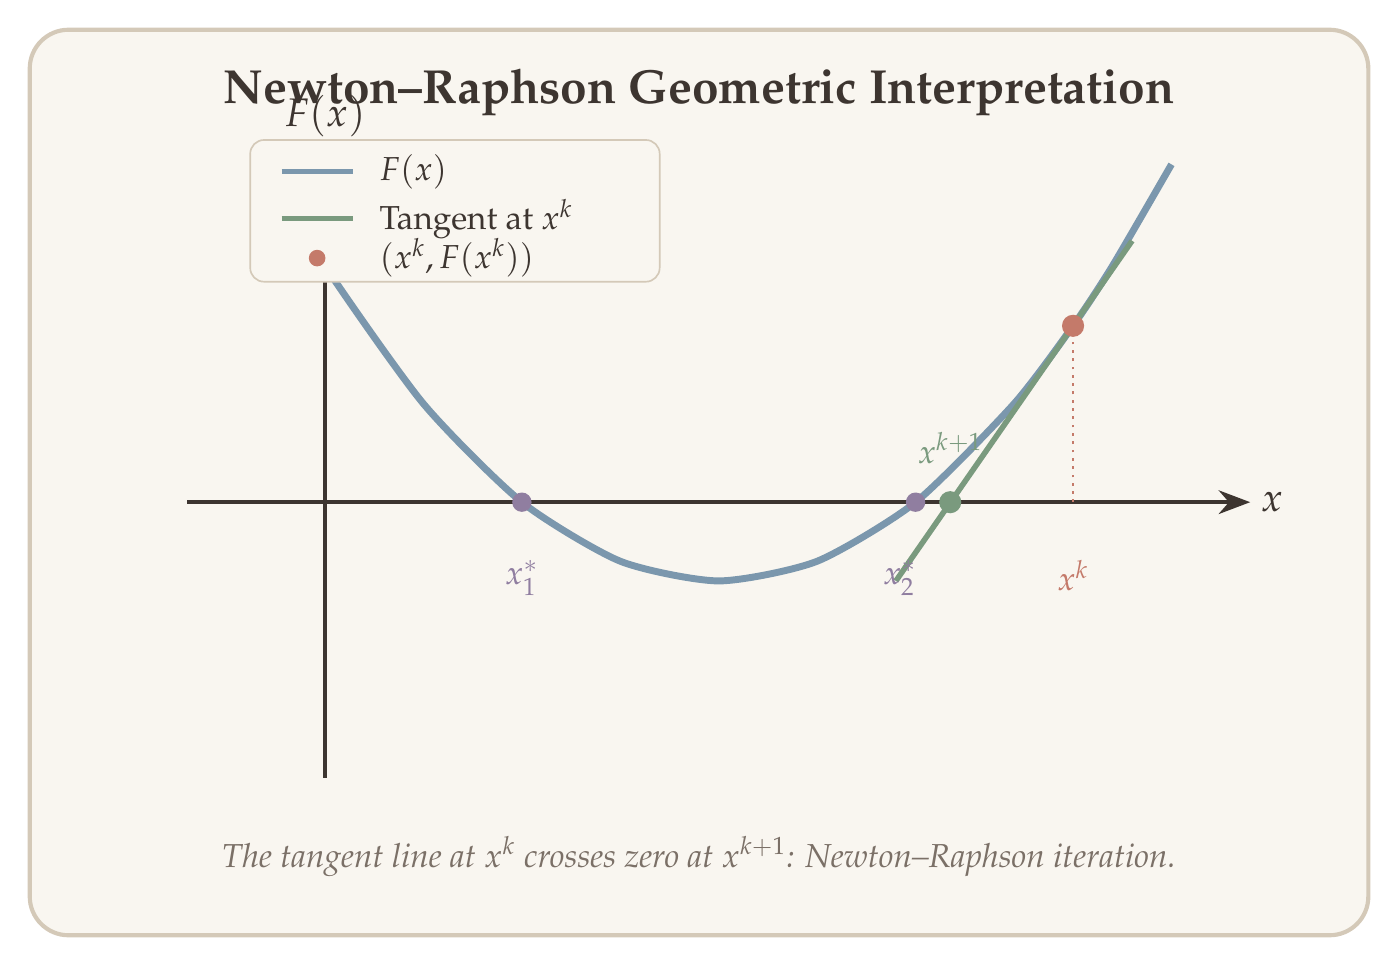
\begin{tikzpicture}[>={Stealth[length=4mm, width=3mm]}, line width=1.5pt]

% Background
\fill[cream, rounded corners=14pt] (-2.5,-2.5) rectangle (14.5,9);
\draw[border, line width=1.5pt, rounded corners=14pt] (-2.5,-2.5) rectangle (14.5,9);

% Title
\node[font=\LARGE\bfseries, text=dkbrown] at (6,8.2)
  {Newton--Raphson Geometric Interpretation};

% Coordinate transform: x in [-0.5,4.5] -> tikz x in [0,12.5] (scale 2.5)
%                        y: tikz y = y_math*2 + 3 (so y=0 is at tikz y=3)
% F(x) = 0.5*(x-1)*(x-3), roots at x=1 (tikz 3.75), x=3 (tikz 8.75)
% Vertex: x=2 (tikz 6.25), F(2)=-0.5 (tikz 2.0)
% x^k = 3.8 (tikz 10.75), F(3.8) = 1.12 (tikz 5.24)
% F'(3.8) = 1.8
% Tangent: y = 1.12 + 1.8*(x-3.8), crosses zero at x = 3.178 (tikz 9.19)

% --- Axes ---
\draw[->, dkbrown, line width=1.5pt] (-0.5,3) -- (13,3)
  node[right, font=\Large, text=dkbrown] {$x$};
\draw[->, dkbrown, line width=1.5pt] (1.25,-0.5) -- (1.25,7.5)
  node[above, font=\Large, text=dkbrown] {$F(x)$};

% --- F(x) curve ---
\draw[stblue, line width=2.5pt] plot[smooth, tension=0.4] coordinates {
  (0.5,7.29) (1.25,6.0) (2.5,4.25) (3.75,3.0) (5.0,2.25)
  (6.25,2.0) (7.5,2.25) (8.75,3.0) (10.0,4.25) (10.75,5.24)
  (11.25,6.0) (12.0,7.29)
};

% --- Tangent line at x^k (clipped to canvas) ---
\begin{scope}
\clip (-1,-1) rectangle (13,8);
\draw[sage, line width=2pt] (8.5,2.0) -- (11.5,6.32);
\end{scope}

% --- Points and labels ---

% Vertical dashed line from x^k to F(x^k)
\draw[terracotta, line width=1pt, dotted] (10.75,3) -- (10.75,5.24);

% Point (x^k, F(x^k))
\fill[terracotta] (10.75,5.24) circle (4pt);

% x^{k+1} on x-axis
\fill[sage] (9.19,3) circle (4pt);

% Root markers
\fill[lavender] (3.75,3) circle (3.5pt);
\node[font=\large, text=lavender, below] at (3.75,2.4) {$x_1^*$};

\fill[lavender] (8.75,3) circle (3.5pt);
\node[font=\large, text=lavender, below] at (8.55,2.4) {$x_2^*$};

% Labels (spaced to avoid overlap)
\node[font=\large, text=terracotta, below] at (10.75,2.4) {$x^k$};
\node[font=\large, text=sage, above] at (9.19,3.35) {$x^{k+1}$};

% --- Legend ---
\fill[cream, rounded corners=5pt] (0.3,5.8) rectangle (5.5,7.6);
\draw[border, line width=0.6pt, rounded corners=5pt] (0.3,5.8) rectangle (5.5,7.6);
\draw[stblue, line width=2pt] (0.7,7.2) -- (1.6,7.2);
\node[font=\large, text=dkbrown, anchor=west] at (1.8,7.2) {$F(x)$};
\draw[sage, line width=2pt] (0.7,6.6) -- (1.6,6.6);
\node[font=\large, text=dkbrown, anchor=west] at (1.8,6.6) {Tangent at $x^k$};
\fill[terracotta] (1.15,6.1) circle (3pt);
\node[font=\large, text=dkbrown, anchor=west] at (1.8,6.1) {$(x^k, F(x^k))$};

% Bottom annotation
\node[font=\large\itshape, text=wmgray] at (6,-1.5)
  {The tangent line at $x^k$ crosses zero at $x^{k+1}$: Newton--Raphson iteration.};

\end{tikzpicture}
\end{document}
